
\chapter{Background}

\section{Maintenance Strategies}

Maintenance strategies are used by companies and organisations to make maintenance decisions about assets, usually machinery \cite{CBM_overview}.
The aim is to keep machines in a state where they can perform tasks as they are required, to a defined standard \cite{CBM_time_prevent}.
Despite the best efforts of designers, machines will always fatigue due to stresses and loads, and will ultimately fail \cite{CBM_overview}.
Failure can be defined in many ways, from breaching performance parameters to complete breakdown, and is specific to the machine and the environment within which it is operating \cite{CBM_overview}.
Organisations which can make better maintenance decisions will make better use of their resources and therefore be more competitive \cite{CBM_overview}.
Costs associated with maintenance vary but can be as high as 70\% in manufacturing, where machine downtime is directly related to output, and represent a large portion of operating budgets across industries \cite{COPM}.
Although maintenance is often viewed through a lens of trying to minimise necessary costs, it can also be a competitive resource \cite{COPM}.
This is especially true when lifetime costs are considered and appropriate marketing strategies are employed \cite{CBM_lifetime}.

\subsection{Corrective and Time-Based Maintenance}

Traditionally, maintenance strategies can be categorised as Corrective Maintenance or Preventive Maintenance (PM) \cite{CBM_time_prevent}.
Corrective Maintenance describes returning machinery to a healthy state, following some failure.
It is also known as run-to-failure and is the simplest maintenance strategy \cite{CBM_time_prevent}.
Although simple and clear, this strategy often results in a lot of downtime, and can result in upstream failures of associated machinery, worsening the impact and cost of failure \cite{CBM_overview}\cite{CM_randall}.
It should be noted that while more complex maintenance strategies will be discussed throughout the rest of this project, failures can never be entirely avoided and Corrective Maintenance will always be required to some degree.
\par

Alternatively, PM describes performing maintenance prior to failure \cite{CBM_overview}.
When maintenance activities are carried out on a regular basis - either in calendar time or operating time - this is known as Time-Based Maintenance (TBM) or scheduled maintenance \cite{CBM_time_prevent}\cite{CM_practical_wind_turbine}.
TBM relies on the assumption that failure can be predicted and is a function of time \cite{CBM_time_prevent}\cite{CM_practical_wind_turbine}.
For mechanical parts, this function is often modelled using the ``Bathtub Curve'' \cite{CM_practical_wind_turbine} (Fig \ref{fig:bathtub}). 
The ``Bathtub Curve'' describes three main sections of the lifetime of a part: burn-in, where the machine is new and adjusts to the environment; useful life, the machine will operate for most of its lifetime in this state, with a low risk of failure; wear-out, the machine has begun to fatigue and the risk of failure is increasing \cite{CM_practical_wind_turbine}.
The principle is that the machine can be maintained as it nears the end of its useful life and therefore the risk of failure remains low.
The practical issue with TBM is that specific data on failure rates of machinery with respect to time can be extremely hard to come by, and may not be available at all for specific applications \cite{CBM_time_prevent}.
Therefore, although the ``Bathtub Curve'' serves as a general model (the `burn-in' period is accounted for by the ISO \cite{ISO17359}) it has limited practical applicability and instead the failure rate is often estimated by experienced engineers \cite{CBM_time_prevent}.
While such expertise can be valuable, the organisation will face problems if such an engineer leaves \cite{CBM_time_prevent}.
Assuming a complete set of failure data is available, TBM dictates an optimisation approach to determine the optimal time interval between maintenance activities on a machine.
Unfortunately, the complex mathematics associated with this approach can be difficult to interpret and are rarely used in practice \cite{CBM_time_prevent}.
\par

While TBM is still a very popular maintenance strategy, it is not the optimal strategy in many cases \cite{CBM_overview}.
There are many opportunities to improve organisational performance and increase profits by implementing more advanced maintenance strategies \cite{CBM_shipping_opportunity}.
This is bolstered by the recent availability of Big Data (BD), which has been shown to increase productivity by 5-6\% when used effectively at large global companies \cite{CBM_norway_bd}.


\begin{figure}
    \centering
    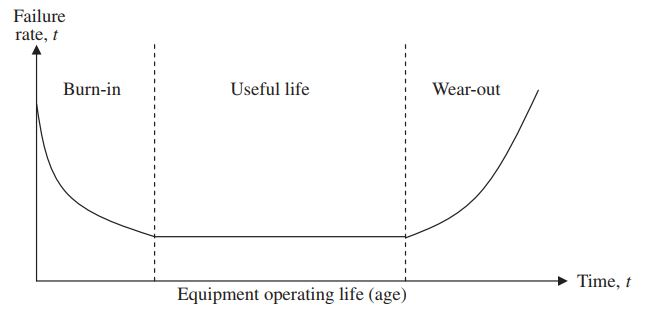
\includegraphics[width=\linewidth]{Bathtub.JPG}
    \caption{Bathtub curve (reproduced from \cite{CBM_time_prevent})}
    \label{fig:bathtub}
\end{figure}

\subsection{Condition Based Maintenance}

Condition Based Maintenance (CBM), also known as Reliability Centered Maintenance (RCM), is a maintenance strategy which requires an understanding of the current and future health of machinery to make maintenance decisions \cite{CBM_overview}.
CBM programs have three key stages:
\begin{enumerate}
    \item Data acquisition
    \item Data processing
    \item Decision making
\end{enumerate}
The grand aim of CBM is to be able to predict when and how a machine will fail, so that maintenance can be performed just before a failure occurs, thereby increasing the efficiency of maintenance activity \cite{CBM_overview}.
Fig \ref{fig:strategies} demonstrates how CBM finds a balance between many maintenance operations and waiting for total failure.
Initially, the greatest gains from CBM were made in settings where machines ran for long periods of time with stable loads \cite{CM_randall}.
Developments in technology have made CBM both more relevant and more practical \cite{CBM_overview}\cite{CBM_norway_bd}.
Systems and machines which require maintenance have become more complex and expensive, while the sensors, processors and algorithms required to implement CBM have become cheaper and more effective \cite{CBM_norway_bd}.
\par

In theory, the exact condition of the machine can be discerned from signals which can be measured externally during operation, such as vibrational and electrical signals \cite{CBM_overview}.
There is extensive literature identifying particular faults in such signals, which will be discussed in more detail in Section \ref{sec:CM}.
\par

As far back as 1978, it was shown that many components and machines fail in a manner that cannot be predicted by age alone \cite{RCM}.
Specifically, an investigation into failure of components on aircraft found that only 11\% showed a distinct wearout zone.
The fact that only a small percentage of components would benefit from the kind of age limits imposed by TBM led to a reform towards CBM within the aviation industry \cite{RCM}.
After a significant delay of 5-10 years, the reliability of aircraft improved significantly, and total passenger fatalities have continued to decrease, even as the number of passengers rises; a clear demonstration of the effectiveness of CBM \cite{CBM_beyond_maritime}.

\begin{figure}
    \centering
    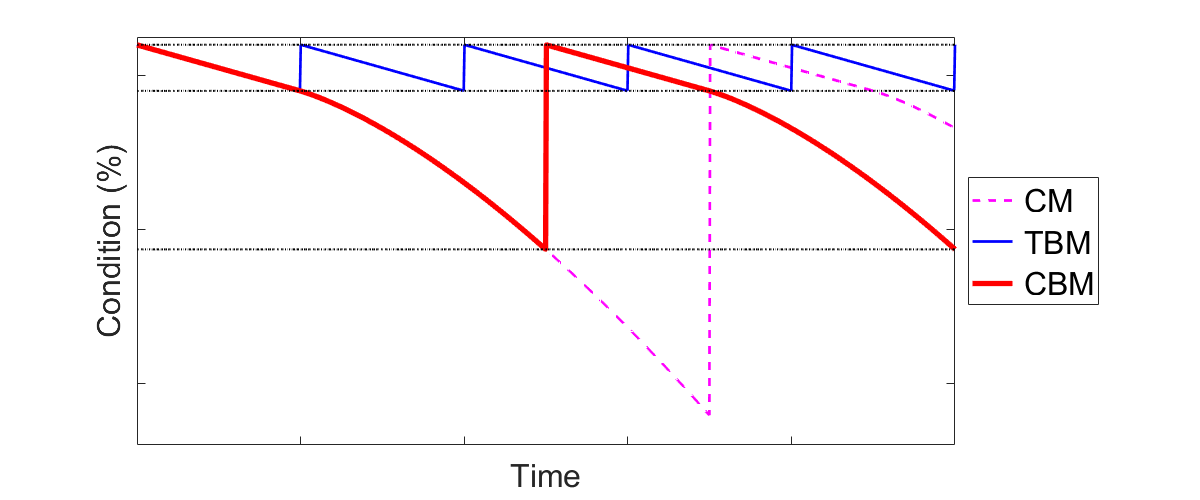
\includegraphics[width=\linewidth]{maintenance.png}
    \caption{Maintenance methods (adapted from \cite{CM_practical_wind_turbine})}
    \label{fig:strategies}
\end{figure}

\subsection{Maintenance in the Maritime Industry}

While CBM has been successfully implemented in many industries the maritime industry has lagged behind \cite{CBM_maritime_ann}.
Costs related to reliability and availability within shipping are estimated at 20 to 30\% of operating costs, yet TBM is still the predominant strategy \cite{CBM_maritime_ann}\cite{Maritime_stopford}.
An investigation by Lloyd's Register found that only 17\% of classified ships operate with an approved Planned Maintenance System, and even fewer operate CBM \cite{CBM_danny}.
The maritime industry is particularly cost focused and so far, the economic considerations have not justified widespread deployment of CBM \cite{CBM_beyond_maritime}\cite{CBM_maritime_ann}.
Notably, the main engines and other parts of the propulsion system are likely to have a Condition Monitoring System (CMS) in place, as their enormous cost and importance to the operation of ships does justify the monitoring cost \cite{CBM_beyond_maritime}.
However, there can be close to 1000 rotating machines on a large ship, most of which have no regular monitoring, and recording of condition and event data is poor \cite{CBM_shipping_opportunity}.
\par

There have been repeated calls for condition monitoring and CBM to play a bigger role in the maritime industry \cite{CBM_shipping_opportunity}\cite{CBM_lr}.
Global competition within ship manufacturing may finally provide the necessary impetus for increased uptake of condition monitoring on board ships \cite{CBM_lifetime}.
By providing lifelong service contracts along with the vessel, ship builders who implement CBM into vessels can compete on quality and lifetime asset cost \cite{CBM_lifetime}.
The advantage to the ship builders is increased sales and a constant revenue stream.
The advantages for the customer are: the likelihood that maintenance costs can be minimised and calculated for by the service contract; service quality is assured across the lifetime of the ship; the customer can focus on their core business.
This business model is currently under trial as part of the EU-funded ThroughLife project \cite{CBM_lifetime}.
\par

Though a novel approach within shipping, other sectors have already developed such models, such as Software-as-a-Service and analytics-as-a-service \cite{CBM_norway_bd}.
These services allows companies to take advantage of BD analytics without necessarily employing experts in-house.
Condition monitoring on ships would provide a source of BD which could be powerful as a prognosis tool (Section \ref{sec:CM_diag}).
Collecting data from a wide range of ships and environments - such as a fleet of vessels - could improve maintainability and influence the design of future vessels \cite{CBM_norway_bd}.\par
It appears that the maritime industry is ready for CBM and stands to benefit from widespread implementation.
However, in a traditionally cost-averse industry, CMSs must have a relatively cheap upfront cost, be accurate, and be introduced alongside business models which offer advantages to ship builders, operators and customers alike \cite{CBM_shipping_opportunity}\cite{CBM_norway_bd}.

\section{Condition Monitoring}\label{sec:CM}

Condition monitoring is the technique which underpins CBM: in order to make maintenance decisions based on the condition of a machine or system, there must be sufficient information about the condition \cite{CM_randall}.
While it is possible to carefully analyse machines after they have broken and thereby isolate the likely failure mechanism, there are a multitude of techniques available for accurately estimating condition during normal operation.
To give a brief list: vibration analysis; motor current signature analysis; oil analysis; thermography; performance analysis; pressure sensing; electrostatic charge sensing; acoustic emissions analysis \cite{CBM_overview}\cite{CM_randall}\cite{CBM_wind_signal}.
Vibration analysis (Section \ref{sec:CM_vib}) is the most widely used method, and Motor Current Signature Analysis (MCSA) (Section \ref{sec:CM_MCSA}) has proven very successful for electric motors.
The common factor between them is that data can be collected repeatedly, on-demand, without interfering with operation and can then be analysed with a variety of signal processing techniques \cite{CM_randall}.


\subsection{Signal Processing Techniques}

Whichever specific data type is chosen, there are an array of processing techniques which can be used to extract useful information.

\subsubsection{Time Domain}

The most basic method available is looking at the data in the time domain \cite{CM_randall}.
Simple parameters such as period, peak, mean and standard deviation can be calculated and used to characterise the waveform \cite{CM_dai_gao_2013}.
More complex measures such as root-mean-square (RMS), skewness, kurtosis have been used to support this characterisation \cite{CM_dai_gao_2013}.
The RMS of vibration velocity is used by the ISO to give numerical limits for machines \cite{ISO10816-7}.
The maximum value and ratio between maximum and RMS can also be indicative of faults related to gearboxes and bearings \cite{VIB_rms}\cite{ISO13373-3}.
\par

Many signals contain a large amount of noise that is not related to the machine under inspection.
The noise can be treated as a random signal and can therefore be removed to some extent through averaging \cite{CM_randall}.
The aim of this is to emphasise the ``true'' signal from the machine, however there are many circumstances in which it will not prove truly effective.
Noise may not be random in nature but emanating from other nearby machinery, and changes in operating condition or load will be misrepresented by averaging \cite{CM_randall}\cite{CM_dai_gao_2013}.
One solution to these issues is order tracking, which uses information about the position of the machine in its cycle to remove the effects of random speed variations \cite{CM_randall}.
Often used with rotating machines, where the angle of the shaft is measured by a tachometer or shaft encoder, data is collected at equal intervals of rotation rather than time.
Order tracking also allows condition monitoring to take place at a variety of speeds for comparison of resonances.
This can then be averaged or processed separately on an angular basis, ensuring that the remaining signal is directly associated with the machine of interest \cite{CM_bonnardot}.
\par

There are also novel techniques such as representing the time signal in a two-dimensional image so that image processing techniques can be applied.
Through a scale invariant feature transform, patterns which are not immediately obvious in the time data can be recognised and used for fault detection and diagnosis \cite{CM_dai_gao_2013}.
\par
Information from the time domain is useful for determining an overall picture of machine condition, however it can be difficult to discern differences in the signal and is not particularly effective at specific diagnosis \cite{CM_randall}.

\subsubsection{Frequency Domain}

\begin{figure}
    \centering
    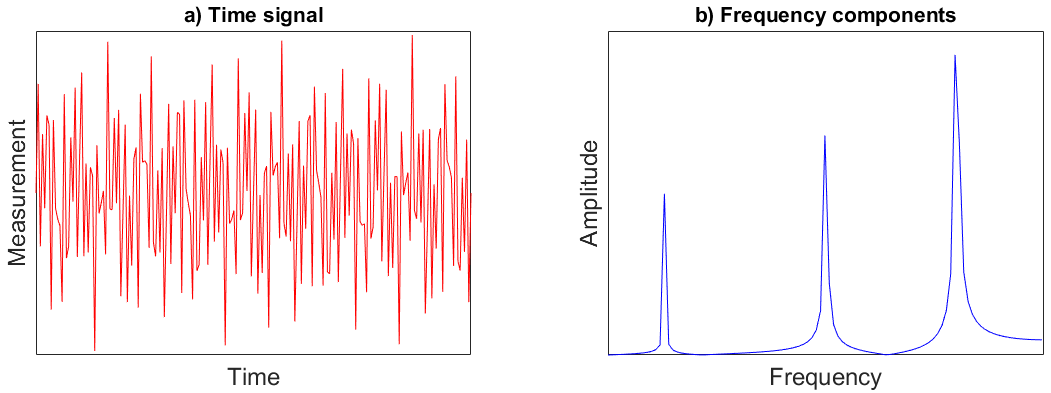
\includegraphics[width=\linewidth]{fourier.PNG}
    \caption{Frequency spectrum of a simple signal via Fourier Transform}
    \label{fig:fourier}
\end{figure}

\begin{figure}
    \centering
    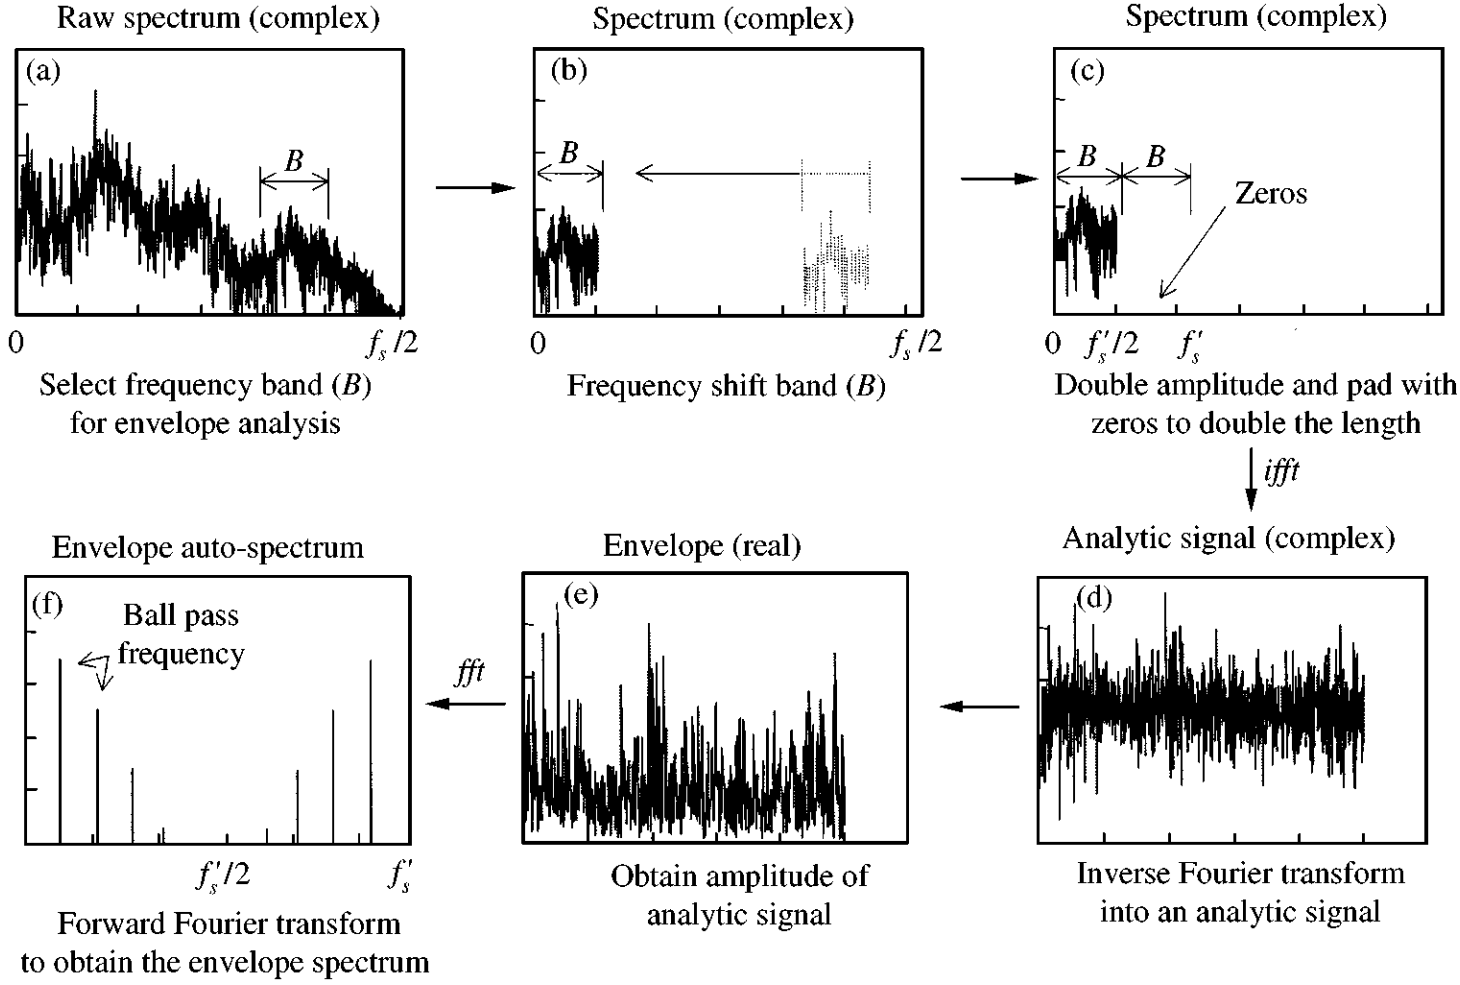
\includegraphics[width=\linewidth]{hilbert.PNG}
    \caption{Hilbert Transform (reproduced from \cite{CM_hilbert})}
    \label{fig:hilbert}
\end{figure}

To efficiently extract information, signals are often transformed to the frequency domain.
The principle is that any periodic signal is composed of the sum of all possible sinusoids, each of which contribute a certain amount of the signal.
Viewing the signal in the frequency domain, the relative input of each frequency can be seen and associated with physical components of the machine \cite{CM_randall}.
\par

This transformation is well-known as the Fourier Transform.
In most modern applications, data is collected at regular intervals (according to the sampling frequency) and therefore the Discrete Fourier Transform (DFT) is used.
For time signal $f$ with $N$ samples, frequency bins $F(k)$ are calculated by:

\begin{equation} %DFT
F(k) = \sum^{N-1}_{n=0} f[n]e^{-2j\pi kn/N}
\end{equation}

DFT is normally performed using a more computationally efficient method, the Fast-Fourier Transform (FFT), of which there are many variants with specific implementation advantages \cite{CM_randall}.
The resolution of the DFT is determined by the sampling rate and the number of samples:
\begin{equation}
    f_{res} = f_{s} / N
\end{equation}
A notable limit on the DFT is the `Nyquist Frequency', which is half the sampling frequency.
Any components in the signal above the Nyquist Frequency will cause errors due to aliasing - appearing as other frequencies.
Therefore, the sampling frequency should be well above twice the maximum frequency component likely to be measured and in practical applications should be higher still.
ISO recommends a frequency range at least 3.5X as high as the largest component of interest \cite{ISO13373-1}.
\par

Taking the magnitude of the DFT frequency bins, which are imaginary numbers, gives the frequency spectrum most commonly seen, with a range from 0 Hz to the Nyquist Frequency (Fig \ref{fig:fourier}).
The shape of this spectrum can be used as a `signature' for certain machine conditions.
Starting from a known healthy condition, it is possible to ascertain how the spectrum changes when faults are introduced to the system \cite{CM_randall}.
In many papers investigating CM, these faults are carefully designed within a laboratory environment, allowing the related components in the frequency spectrum to be identified.
The identified components can then be focused on during monitoring machines operating outside of the laboratory.
\par

Large amounts of noise can affect the frequency spectrum \cite{CM_randall}.
Averaging the frequency spectrum over time makes the consistent frequency components clearer, at the cost of diminishing the effect of impulses, which are associated with particular faults and often appear in the higher frequency bands \cite{CM_randall}.
To remove discrete and random noise around a specific band of frequencies, envelope analysis is performed with the Hilbert Transform \cite{CM_hilbert}.
Known as demodulation, this process allows impulses in the signal to be detected much more easily than in the original signal.
The frequency band of interest is usually related to a resonance in the machine \cite{CM_bonnardot}.
The procedure is described in Fig \ref{fig:hilbert}.
Note that the inverse-Fourier transform and Fourier transform performed in steps d) and f) are performed on signals with a much smaller length than the original signal and therefore do not add significantly to the computational workload \cite{CM_hilbert}.
The Hilbert transform has been combined with a statistical model to identify roller bearing faults in the challenging environment of a helicopter gearbox, although limitations at high frequencies were noted \cite{CM_hilbert}.
\par

Literature detecting and diagnosing faults in the frequency domain is abundant and continues to be a primary tool for CBM.
It provides a clear technique for taking advantage of \textit{a priori} knowledge of the machine, as calculated frequencies can be compared directly to the measured signal \cite{CM_dai_gao_2013}.
Transforming to the frequency domain is no longer a computational obstacle and provides relevant information for both users and data-driven methods \cite{CM_randall}.
A large number of condition monitoring systems employ frequency analysis and specific recommendations are provided by the ISO \cite{CM_list_wind_CMS}\cite{ISO13373-1}.


\subsubsection{Time-Frequency Domain}

\begin{figure}
    \centering
    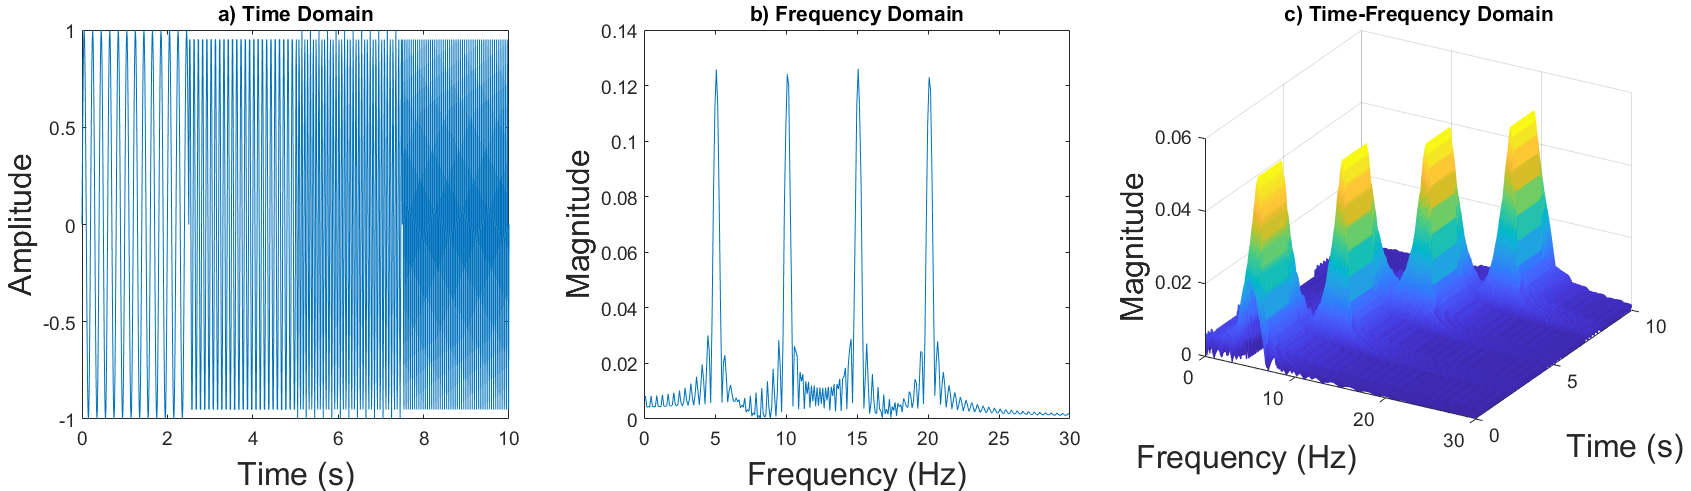
\includegraphics[width=\linewidth]{stft.png}
    \caption{Viewing a signal which changes in time in multiple domains}
    \label{fig:stft}
\end{figure}

The Time-Frequency Domain is seeing wider use with recent increases in computing power making it more practical.
Its purpose is to capture how the frequency spectrum changes with respect to time \cite{CM_dai_gao_2013}.
This is particularly useful for detecting impulses and other high frequency signals \cite{wavelet_tut}.
The challenge in obtaining such information stems from the uncertainty principle, which states that exact information cannot be known about the time and frequency simultaneously \cite{wavelet_tut}.
While the DFT provides excellent information about the frequency components of the signal, all information about how the signal changes in time is lost.
Conversely, the time-domain contains no frequency information.
Fig \ref{fig:stft} demonstrates how a signal with different frequencies at different times can be misinterpreted in the frequency domain but seen much more clearly in the time-frequency domain.


\par
The Short-Time Fourier Transform (STFT) is a method for transforming a time signal to the time-frequency domain \cite{CM_dai_gao_2013}.
DFT is applied to windows of the signal in time.
Formally, the STFT of a signal ${x(t)}$ is calculated as:
\begin{equation*}
STFT_x(t, \omega) = \frac{1}{\sqrt{2\pi}}\int^{+\infty}_{-\infty}x(\tau)h(\tau-t)e^{-j\omega \tau}d\tau
\end{equation*}
where $h(\tau)$ the windowing function.
Windowing splits the time signal up into a smaller signal, with weights applied to the time samples to reduce the `picket-fence' effect which causes distortions in the frequency-domain \cite{CM_randall}.
For simple computation, a rectangular window can be applied - where all samples within the window are weighted equally - but  Hanning and Gaussian windows are the most common \cite{CM_dai_gao_2013}.
As it involves performing DFT at many time steps, STFT is much more computationally intensive than DFT, while still being quicker than other time-frequency transformations.
The STFT also provides output in familiar units for time and frequency and as such is highly readable by humans for analysis \cite{wavelet_tut}\cite{CM_wavelets}.
Although it has been widely used for CM, STFT has been found to give poor results for non-stationary signals and so is not suitable for many applications, particularly tool wear \cite{CM_wavelets}.
\par

Wavelet Analysis (WA) was developed to improve on the time-frequency information provided by the STFT by taking advantage of multi-resolultion analysis \cite{wavelet_tut}\cite{CM_wavelets}.
There are similarities in the technique, but WA relies on wavelets, which are chosen with particular properties to increase accuracy \cite{CM_wavelets}.
WA minimises the time error of high frequency signals and the frequency error of low frequency signals \cite{wavelet_tut}.
This is in contrast to STFT, which provides constant distribution errors across time and frequency \cite{CM_wavelets}.
The Continuous Wavelet Transform (CWT) of $x(t)$ is calculated with:
\begin{equation*}
  CWT_x(a, b) = \frac{1}{\sqrt{\abs{a}}}\int^{+\infty}_{-\infty}x(t)\psi*\left(\frac{t-b}{a}\right)dt\;a, b\in \mathbb{R}
\end{equation*}
where $a$ and $b$ are parameters associated with frequency and time respectively \cite{CM_waveletVsFourier}.
WA is more computationally intensive than STFT and results of WA are not readable directly in time and frequency units \cite{CM_wavelets}.
Despite these drawbacks, it has become a widespread technique in condition monitoring and other domains \cite{CM_dai_gao_2013}.
\par

WA is used for denoising non-stationary signals in the time and frequency domain simultaneously \cite{CM_randall}.
Once the signal has been transformed to the time-signal domain, there often only remain a small number of large coefficients and thresholding is applied, removing coefficients below a certain level.
The inverse transform can then be applied, providing a signal with significantly less noise for further analysis \cite{CM_wavelets}.
\par

Further evidence of the versatility of WA is provided by its use in denoising and multiresolution feature extraction of Electrocardiogram (ECG) signals \cite{CM_wavelet_ecg}.
Through the lens of this paper, WA proved a valuable tool for CM of the brain using noisy, non-stationary signals.
\par

Time-frequency domain analyis is becoming more common, however the increased computational complexity compared to time and frequency domain analysis is significant \cite{CM_randall}.


\subsection{Fault Detection and Diagnostics (FDD)}\label{sec:CM_diag}

Another important component of CBM is the ability to detect and diagnose faults as they occur.
While the ISO gives recommendations on how overall vibration levels are related to machine health, being able to diagnose the fault with respect to specific components provides a significant advantage when making maintenance decisions \cite{ISO10816-7}\cite{CM_mcsa_vib}.
In an overview of this topic, Dai and Gao \cite{CM_dai_gao_2013} highlight three main categories of fault detection and diagnosis:

\begin{enumerate}
    \item Model-based online - Developing state space models and detecting how parameters move away from their expected values
    \item Signal-based - Monitoring how the measured outputs of a system change and correlating with known fault patterns
    \item Knowledge-based - Using large amounts of historical data to find patterns and correlations
\end{enumerate}

Each of these approaches relies on having accurate and useful data about the system.
The next two sections will provide more in-depth descriptions of the two most successful FDD methods: vibration analysis (\ref{sec:CM_vib}) and MCSA (\ref{sec:CM_vib}) \cite{CM_mcsa_vib}.
The main advantages of both techniques over the other available options are the  relative ease of implementation on a wide range of machines, clear analytical models and data which can be analysed with a variety of methods \cite{CM_dai_gao_2013}\cite{CM_mcsa_vib}.
A brief overview of the differences between the techniques can be seen in Table \ref{tab:mcsa_vib}.
It is clear that not all faults can be detected with MCSA or vibration analysis alone.
For example: vibration analysis cannot identify specific faults with the power supply frequency or individual phases; MCSA cannot identify which bearing is faulty along a shaft.
While MCSA can provide very specific information on induction motors, varying the load on the motor can provide similar signals to some mechanical faults \cite{CM_mcsa_vib}.
Combining the two methods provides coverage of most faults, redundancy of the CMS and allows for specific fault diagnostics \cite{CM_mcsa_vib}\cite{VIB_wireless_sensor}\cite{VIB_MCSA_comb}.
\par

Methods targeting accurate prognosis will be discussed in \ref{sec:prog}.

\begin{table}
	\begin{center}
		\begin{tabular}{lcc}%Changed c to S
			\toprule
			  & \textbf{MCSA} & \textbf{Vib} \\
			\midrule
			Easy radial rotor displacement interpretation & $\checkmark$ & $\times$ \\
			Detecting electrical faults & $\checkmark$ & $\times$ \\
			Applicable in rough environments & $\checkmark$ & $\times$ \\
			Cheap implementation & $\checkmark$ & $\times$ \\
			Early stage mechanical fault detection & $\times$ & $\checkmark$ \\
			Distinguish between several bearings in drive train & $\times$ & $\checkmark$ \\
			Knowledge of mean time to failure determination & $\times$ & $\checkmark$ \\
			Favourable noise to signal ration & $\times$ & $\checkmark$ \\
			\bottomrule
		\end{tabular}
		\caption{MCSA vs Vibration (adapted from \cite{CM_mcsa_vib})}
		\label{tab:mcsa_vib}%Can be referenced by rest of document
	\end{center}
\end{table}

\subsection{Vibration Analysis}\label{sec:CM_vib}

\begin{table}
    \renewcommand{\arraystretch}{1.4}
	\begin{center}
		\begin{tabularx}{\textwidth}{XcX}%Changed c to S
			\toprule
			\textbf{Fault} & \textbf{Frequency} & \textbf{Notes/Causes} \\
			\midrule
			Unbalance, misalignment and bent shaft & $k.f_r$ & Related and appear strongly at the first few multiples of $f_r$ \\
			Oil whip & $0.6 - 0.95f_r$ & Most common fault to appear in the subharmonic range \\
			Bearing inner race (BPFI)& $\frac{k.f_{r}.n}{2}(1+\frac{d}{D}cos\beta)$ & Defect on inner race \\
			Bearing outer race (BPFO)& $\frac{k.f_{r}.n}{2}(1-\frac{d}{D}cos\beta)$ & Defect on outer race\\ 
			Ball spin frequency (BSF) & $\frac{k.f_{r}.d}{2D}(1-(\frac{d}{D}cos\beta)^2)$ & Defect on rolling element \\
			Bearing cage (FTF) & $\frac{k.f_{r}}{2}(1-\frac{d}{D}cos\beta)$ & Defect on cage\\
			Insufficient clearance and expansion of rolling elements & $2\times BSF$ & Bearings can overheat due to improper installation and loading \\
			Lubrication defect & 8 kHz octave band & Can cause bearings to heat up \\
			Contamination & 8 kHz octave band & Abrasion of bearings and inner surfaces \\
			Looseness of bearing housing & Shocks at $f_r$ & Housing is not correctly sized or excessive loading\\
			Unbalanced power supply voltages & $2f_s \pm \frac{1}{3}f_s$ & Can result from loose connections \\
			
			\bottomrule
		\end{tabularx}
		\caption{Faults which can be detected with vibration analysis - mechanical rotor frequency $f_r$, integer $k = 1, 2, 3...$, number of rolling bearings $n$, ball diameter $d$, pitch diameter $D$, bearing contact angle $\beta$, supply frequency for electric motors $f_s$ \cite{CM_randall}\cite{CM_mcsa_vib}\cite{ISO13373-3}\cite{ISO13373-9}}
		\label{tab:vibfaults}%Can be referenced by rest of document
	\end{center}
\end{table}

Vibration analysis takes advantage of the fact that many faults within a rotating machine can be detected and identified from vibration signals produced by the machine.
This information can be extracted by measuring displacement, velocity or acceleration \cite{CM_randall}.
It is generally viewed as the most reliable and widely used condition monitoring method \cite{CM_mcsa_vib}.
\par

An important factor in the efficacy of vibration analysis is the mounting location and method \cite{Smart_Bearings_1}.
Fig \ref{fig:Accelerometer_Locations} shows ISO recommended mounting points for vibration transducers on horizontal pumps.
Increasing the number of sensors on a machine helps to build a more complete picture of machine health.
Using multiple vibration sensors can provide information about the location of faults, for example indicating which bearing is most likely to be faulty \cite{CM_mcsa_vib}.
Additionally, it is essential that the sensors are strongly fixed to their mounting points to accurately measure vibrations \cite{Smart_Bearings_1}.
Screw and stud fittings are the best options as they will perform well in challenging conditions and do not significantly affect the vibration experienced by the sensors \cite{Smart_Bearings_1}.
\par

Table \ref{tab:vibfaults} provides a compilation of faults which can be detected using vibration analysis and the frequencies at which they occur.
The frequencies of interest are usually up to 10 kHz \cite{CM_randall}.
In general, as machines begin to wear and degrade, the overall vibration level increases and can be described by the RMS of vibration data in the time domain \cite{ISO13373-1}.
In some instances, measuring how RMS of velocity or acceleration changes over time is the only processing performed for CBM.
The ISO provide guidance on absolute RMS limits for different categories of machinery \cite{ISO10816-7}.
However, RMS is not suitable for detecting short-lived signals associated with gear tooth or bearing failure \cite{VIB_rms}.
\par

As the most common failure cause for rotating machines, bearing faults are widely investigated in the literature \cite{CM_mcsa_vib}\cite{ISO13373-9}\cite{VIB_distributed_bearing}.
Envelope analysis has proven effective across a range of experiments for detecting specific bearing faults \cite{CM_randall}\cite{VIB_distributed_bearing}\cite{VIB_basic_bearing}.
The ISO provide a chart for comparing the severity of bearing faults (Fig \ref{fig:ISO_bearing}).
If the maximum acceleration is much higher than the expected value based on RMS, it is likely a result of impulses which result from faults on the bearing or gearbox.
This chart is a simple but effective method for identifying bearing failures.
\par
Work on incorporating machine learning into vibration analysis has shown that a few simple statistics can be used to classify the condition of the machine \cite{VIB_moosavian}.
Using only the maximum, RMS and std of the frequency spectrum, an adaptive neuro-fuzzy inference system was trained to differentiate between the healthy condition and two fault conditions (Fig \ref{fig:Moosavian_Figures}).
Large amounts of data were required for training and testing (100s at 8192 Hz for each condition) and proved very accurate.
Notably, training and testing was all performed offline on a computer.
This method could be extended to classify other faults.

\begin{figure}
    \centering
    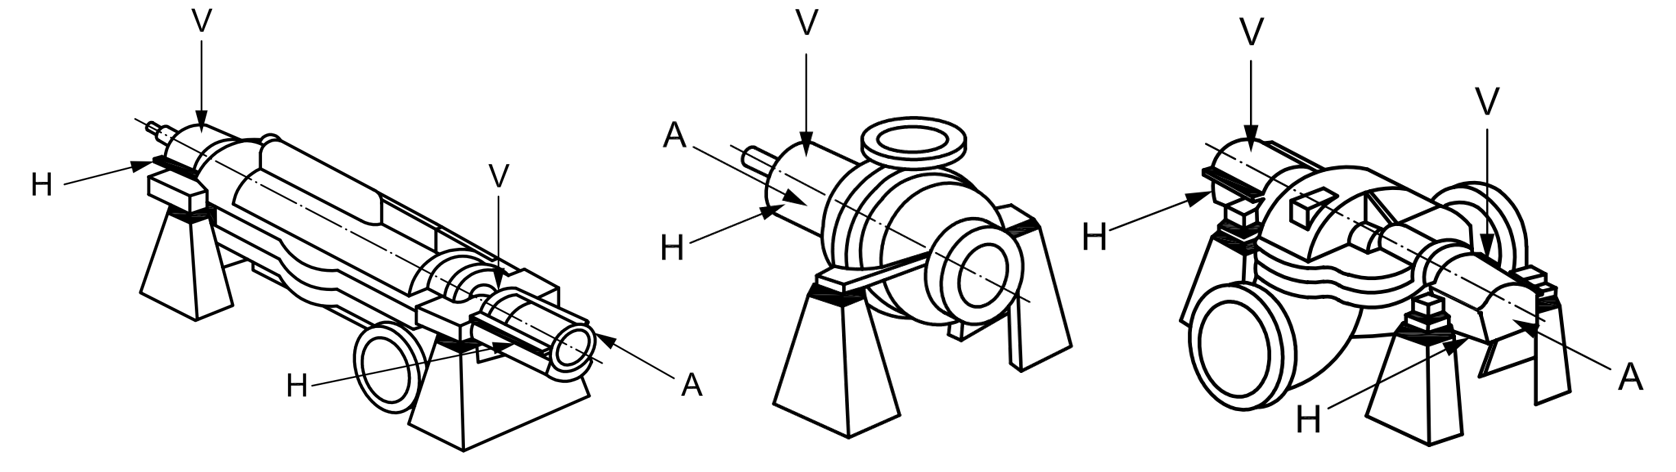
\includegraphics[width=\linewidth]{AccelerometerLocations.PNG}
    \caption{Recommended mounting points for vibration transducers, adapted from \cite{ISO10816-7}}
    \label{fig:Accelerometer_Locations}
\end{figure}

\begin{figure}
    \centering
    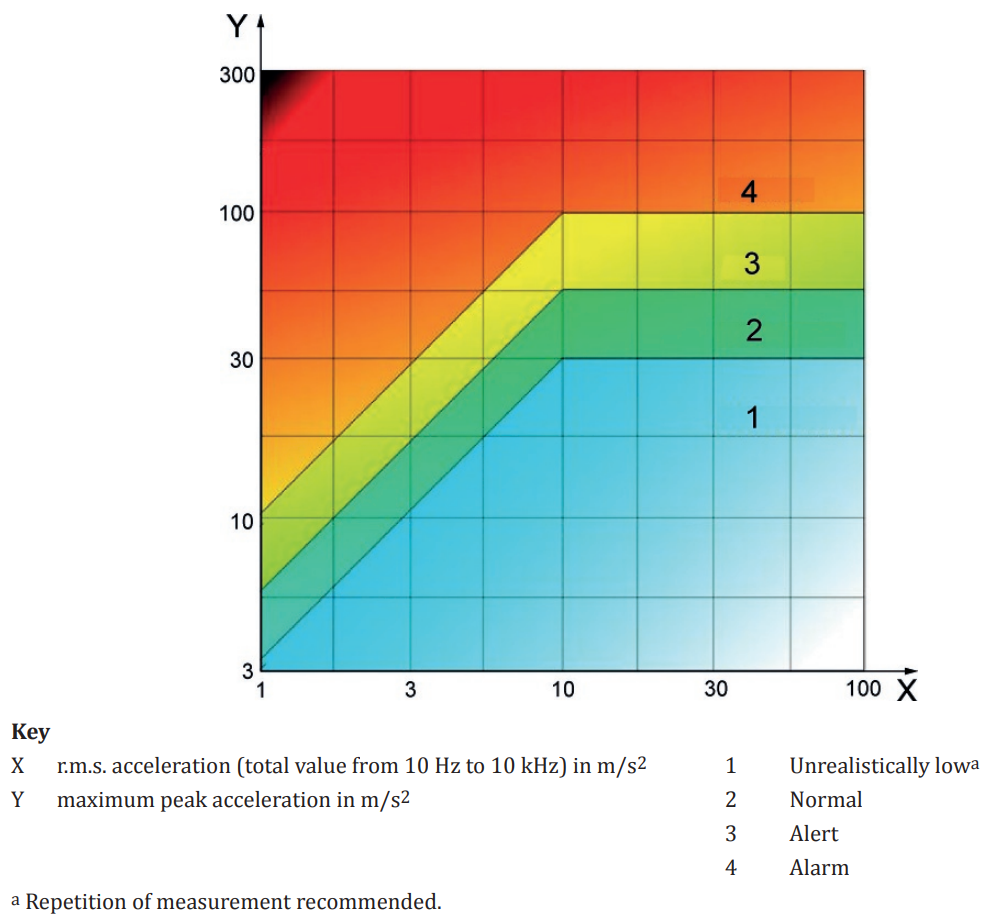
\includegraphics[width=\linewidth]{ISO_bearing.PNG}
    \caption{Bearing fault severity chart, reproduced from \cite{ISO13373-3}}
    \label{fig:ISO_bearing}
\end{figure}

\begin{figure}
  \centering
  \begin{subfigure}[b]{0.49\textwidth}
    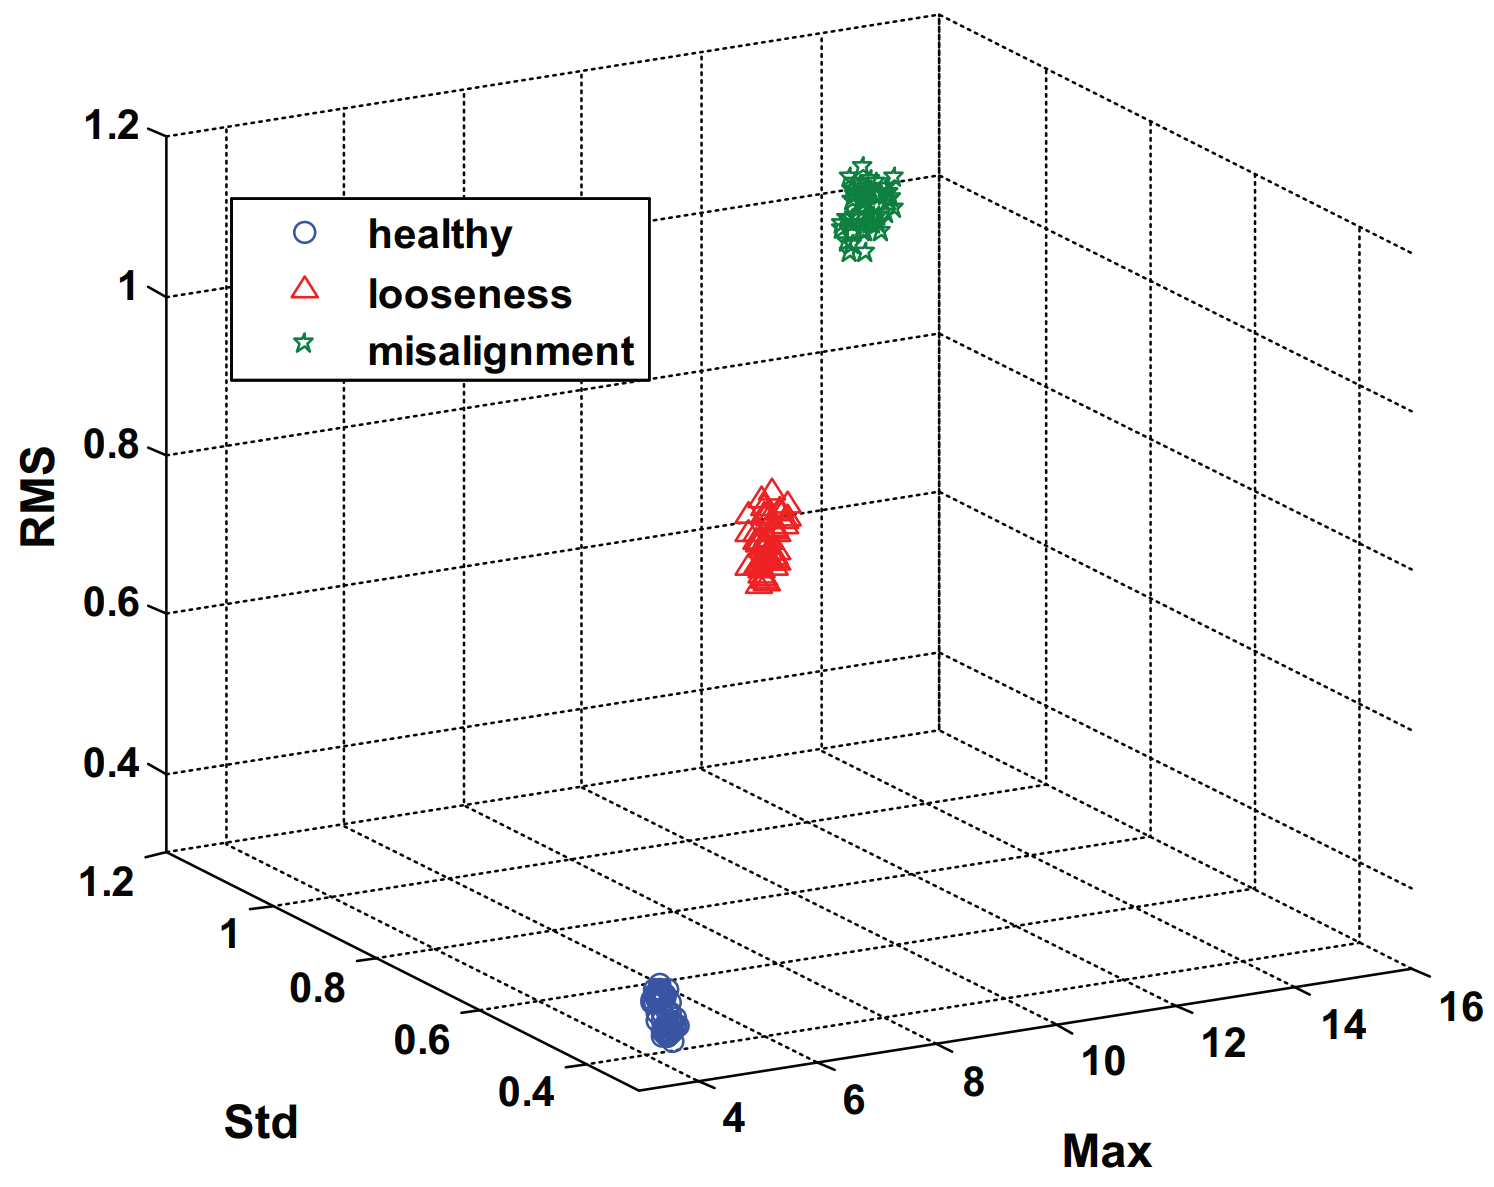
\includegraphics[width=\linewidth]{Moosavian1.PNG}
    \caption{Statistical features}
  \end{subfigure}
  \begin{subfigure}[b]{0.49\textwidth}
    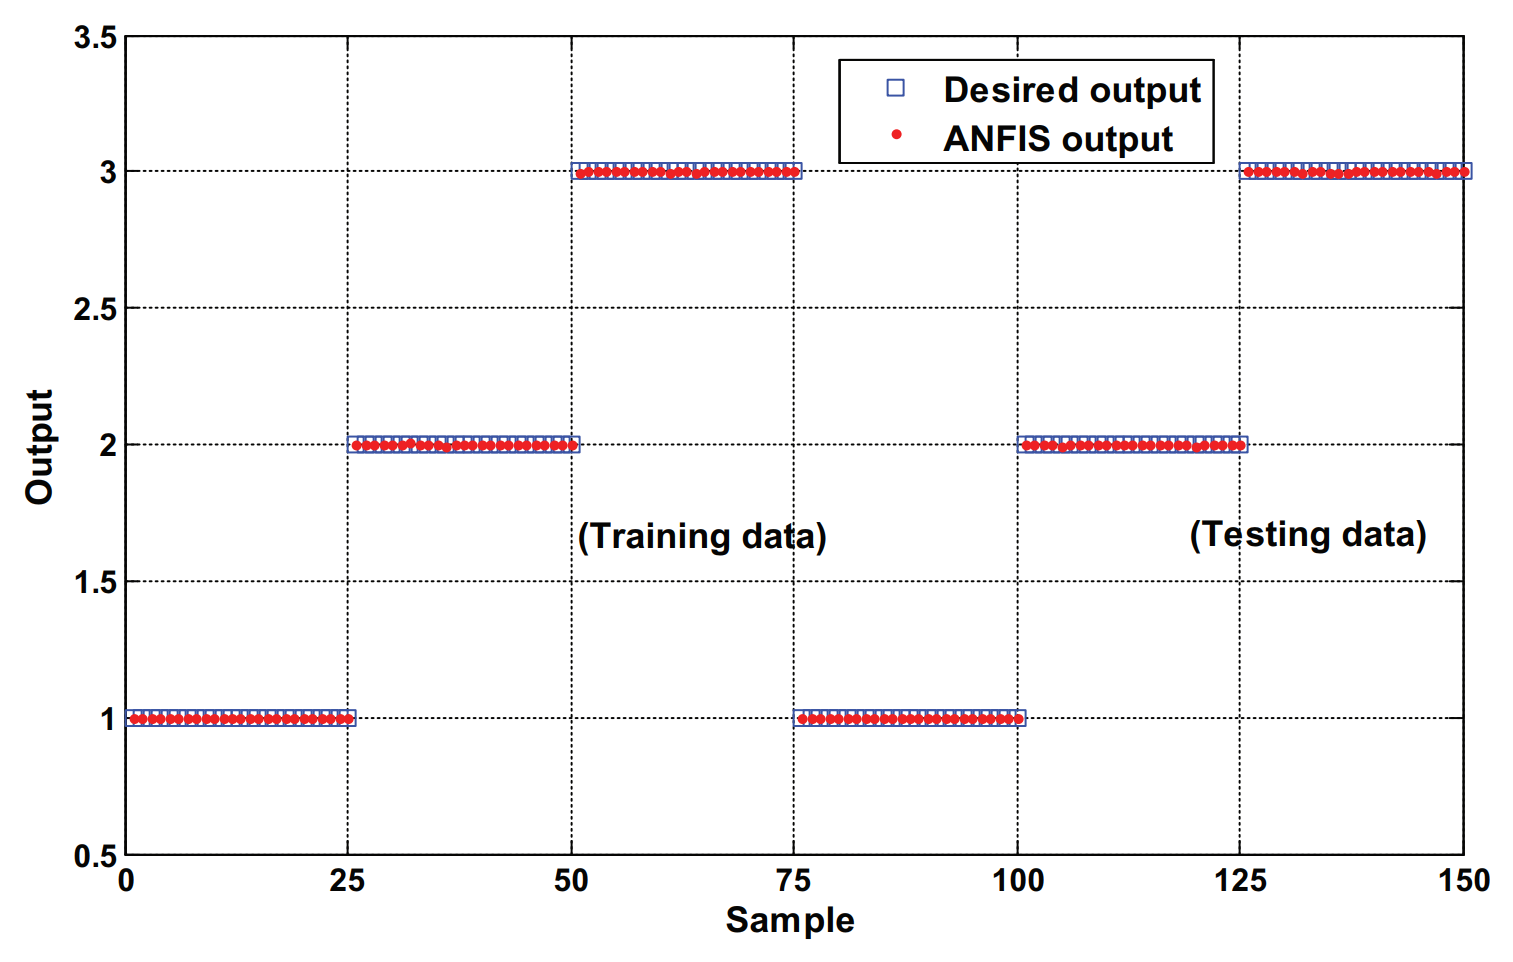
\includegraphics[width=\linewidth]{Moosavian2.PNG}
    \caption{Classification results}
  \end{subfigure}
  \caption{Implementation of ANNs with fuzzy logic for classification of water pump condition, reproduced from \cite{VIB_moosavian}}
  \label{fig:Moosavian_Figures}
\end{figure}


\subsection{Motor Current Signature Analysis}\label{sec:CM_MCSA}

\begin{figure}
  \centering
  \begin{subfigure}[b]{0.45\textwidth}
    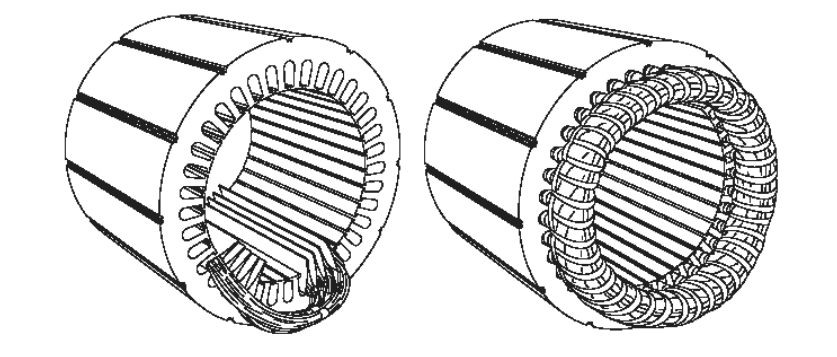
\includegraphics[width=\linewidth]{Stator_Diagram.PNG}
    \caption{Typical stator}
  \end{subfigure}
  \begin{subfigure}[t]{0.54\textwidth}
    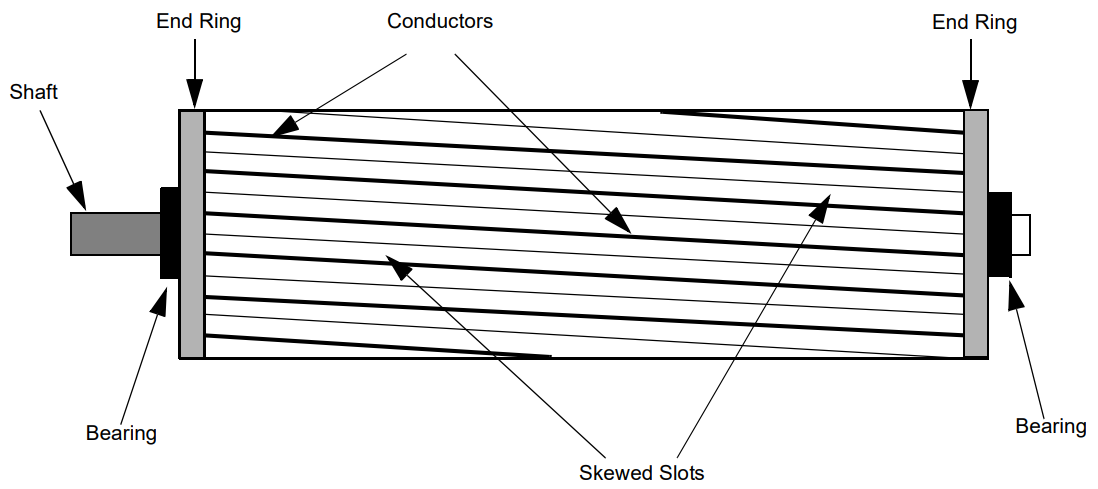
\includegraphics[width=\linewidth]{Rotor_Diagram.PNG}
    \caption{Typical squirrel cage rotor}
  \end{subfigure}
  \caption{Typical elements of a squirrel cage induction motor, reproduced from \cite{Squirrel_Cage_Tutorial}}
  \label{fig:Squirrel_Cage_Diagram}
\end{figure}

\begin{table}
    \renewcommand{\arraystretch}{1.4}
	\begin{center}
		\begin{tabularx}{\textwidth}{XcX}%Changed c to S
			\toprule
			\textbf{Fault} & \textbf{Frequency} & \textbf{Notes/Causes} \\
			\midrule
			Shorted stator winding & $v.f_s \pm k.f_r$ & Short circuit in stator windings  \\
			Broken rotor bar & $f_s \pm 2.k.s.f_s$ & Motor can fail if numerous enough \\
			Static rotor eccentricity & $v.f_s \pm k.RS.f_r$ & Air gap eccentricity which can be very damaging to the motor\\
			Dynamic rotor eccentricity & $v.f_s \pm (k.RS\pm n).f_r$ & Air gap eccentricity\\
			Mixed rotor eccentricity & $f_s \pm k.f_r$ & Air gap eccentricity\\
			BPFI & $f_s \pm k.fr\frac{n}{2}(1+\frac{d}{D}cos\beta)$ & Defect on inner race\\
			BPFO & $f_s \pm k.fr\frac{n}{2}(1+\frac{d}{D}cos\beta)$ & Defect on outer race\\
			BSF & $f_s \pm \frac{k.f_{r}.d}{2D}(1-(\frac{d}{D}cos\beta)^2)$ & Defect on rolling element \\
			FTF & $f_s \pm \frac{k.f_{r}}{2}(1-\frac{d}{D}cos\beta)$ & Defect on cage\\
			\bottomrule
		\end{tabularx}
		\caption{Faults which can be detected with MCSA - mechanical rotor frequency $f_r$, supply frequency $f_s$, slip $s$, number of rotor slots RS, integers $k, n = 1, 2, 3..., v = 1, 3, 5...$, number of rolling bearings $n$, ball diameter $d$, pitch diameter $D$, bearing contact angle $\beta$, \cite{CM_mcsa_vib}\cite{ISO20958}}
		\label{tab:mcsafaults}%Can be referenced by rest of document
	\end{center}
\end{table}

\begin{figure}
    \centering
    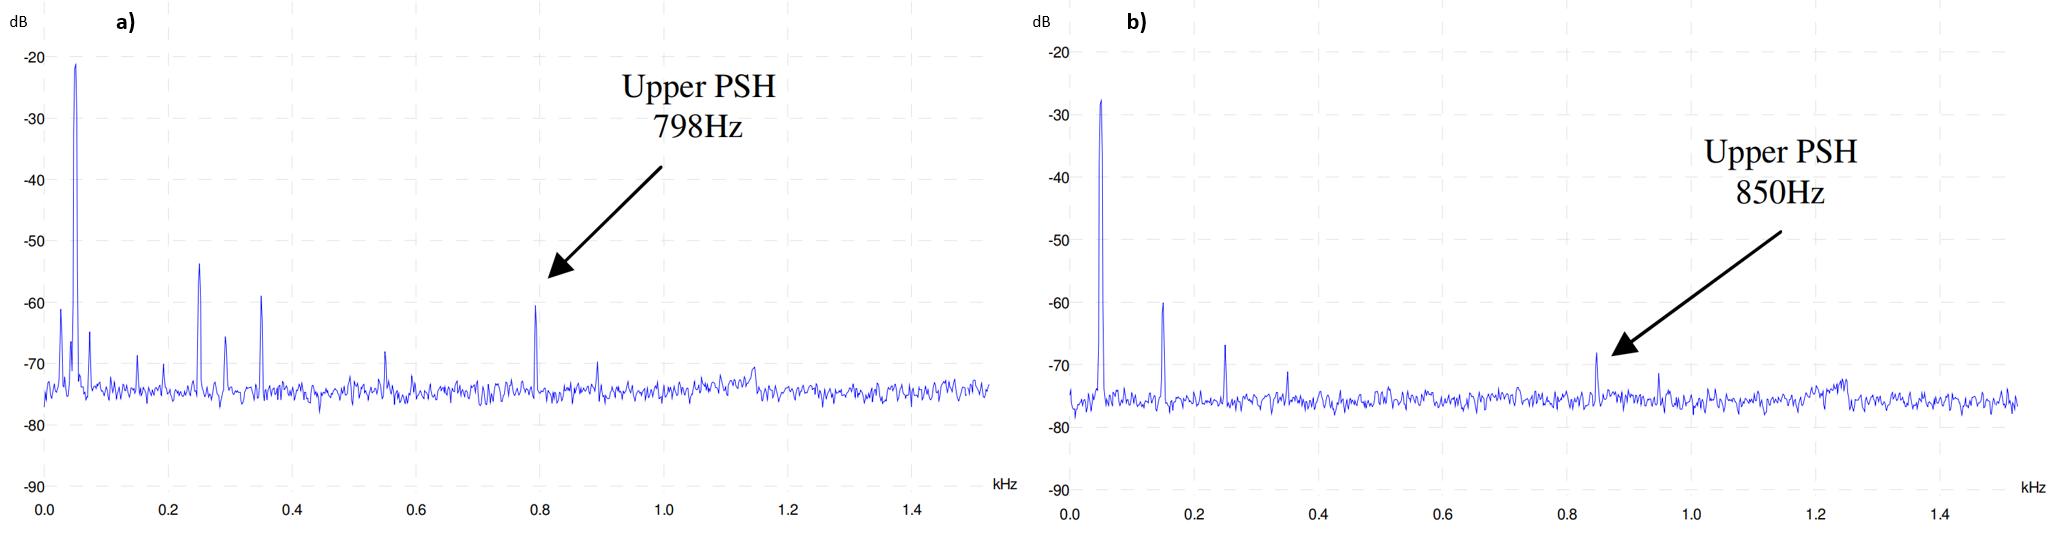
\includegraphics[width=\linewidth]{MCSA_healthy.PNG}
    \caption{Healthy current signal for cage rotor induction motor with 36 slots, 32 bars and 2 pole pairs for a) loaded, slip = 6.4\% b) unloaded, slip = 0, reproduced from \cite{MCSA_healthy_signal}}
    \label{fig:MCSA_healthy}
\end{figure}


For electric motors, MCSA is an extremely powerful tool, and can be used to detect and diagnose faults which are not detectable by vibration alone.
However, healthy behaviour, such as changing loads, can appear similar to faults so care must be taken in application \cite{CM_mcsa_vib}.
MCSA has a long history of usage which has shown that it is versatile and effective \cite{MCSA_case_studies}.
\par

Induction motors are the most numerous motors for industrial systems, with a common design being the three-phase rotor cage induction motor \cite{Squirrel_Cage_Tutorial}.
The two main components are the stator, which remains stationary, and rotor, which rotates (Fig \ref{fig:Squirrel_Cage_Diagram}).
Around half the failures of induction motors are associated with faults on these two components, with another significant portion related to bearing failures \cite{MCSA_case_studies}.
\par

The radial displacement induced by faults causes the air-gap between the rotor and the stator to vary, changing the reluctance and flux linkage.
This can be detected through the stator current \cite{CM_mcsa_vib}.
Electrical faults also have a direct impact on the stator current \cite{MCSA_Review_Benbouzid}.
The stator current can be measured by placing a current sensor around the motor supply cable of a single phase \cite{ISO20958}.
The sensor does not have to be located close to the motor or power supply to measure accurately, providing an advantage over vibrational analysis \cite{CM_mcsa_vib}.
\par

The frequency spectrum is widely used to detect and diagnose faults in MCSA \cite{MCSA_Review_Benbouzid}.
A peak at the supply frequency is expected and can be calculated by:
\begin{equation}
    f_s = N_s \times \frac{120}{P}
\end{equation}
where $N_s$ is the synchronous speed of the motor in RPM and $P$ is the number of poles on the stator \cite{Squirrel_Cage_Tutorial}.
This peak can be seen clearly at 50 Hz in the loaded and unloaded tests shown in Fig \ref{fig:MCSA_healthy}.
\par

As seen from the list of fault frequencies in Table \ref{tab:mcsafaults}, many of the fault frequencies are similar to their vibrational counterparts but centred on the supply frequency \cite{CM_mcsa_vib}.

\par

A technique known as Park's Vector provides diagnosis through the time domain for three-phase motors \cite{MCSA_Parks}.
The three-phase currents ($i_A, i_B, i_C$) are used to calculated the Park's Vector components:
\begin{align}
    i_D &= (\sqrt{2}/\sqrt{3})i_A - (1/\sqrt{6})i_B - (1/\sqrt{6})i_C\\
    i_Q &= (1/\sqrt{2})i_B - (1/\sqrt{2})i_C
\end{align}
In ideal conditions, plotting the values of $i_D$ and $i_Q$ which correspond in time will give a circular locus centred at the origin.
Faults such as shorted turns in the stator winding and broken rotor bars will distort the locus in its shape and thickness respectively (Fig \ref{fig:ParksVector}) \cite{MCSA_Parks}\cite{MCSA_Parks2}.
This method has been enhanced by work showing that the frequency spectrum of the Park's Vector modulus can be more effective for fault detection than simple FFT of the time signal \cite{MCSA_Parks_Extended}.
The cost of this method is more sensors and computational effort to monitor three phases simultaneously.

\begin{figure}
  \centering
  \begin{subfigure}[b]{0.285\textwidth}
    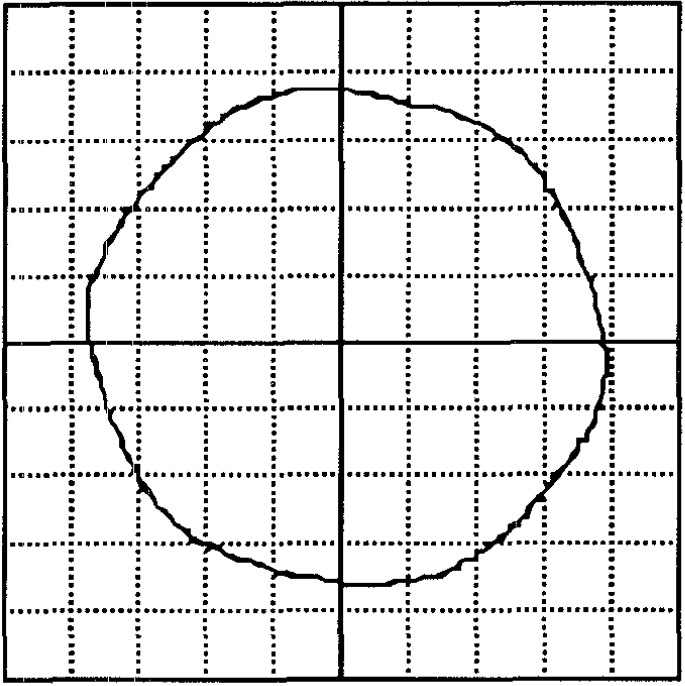
\includegraphics[width=\linewidth]{Parks1.PNG}
    \caption{Healthy}
  \end{subfigure}
  \begin{subfigure}[b]{0.294\textwidth}
    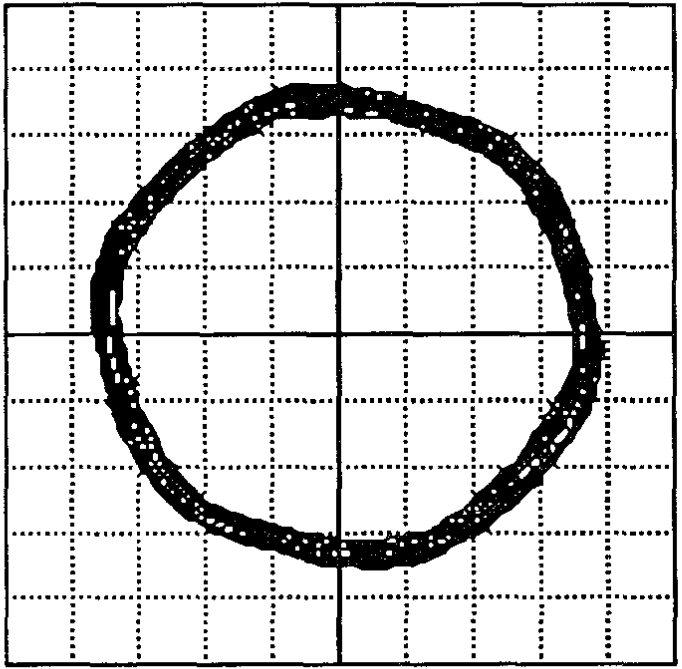
\includegraphics[width=\linewidth]{Parks2.PNG}
    \caption{Broken Rotor Bars}
  \end{subfigure}
  \begin{subfigure}[b]{0.285\textwidth}
    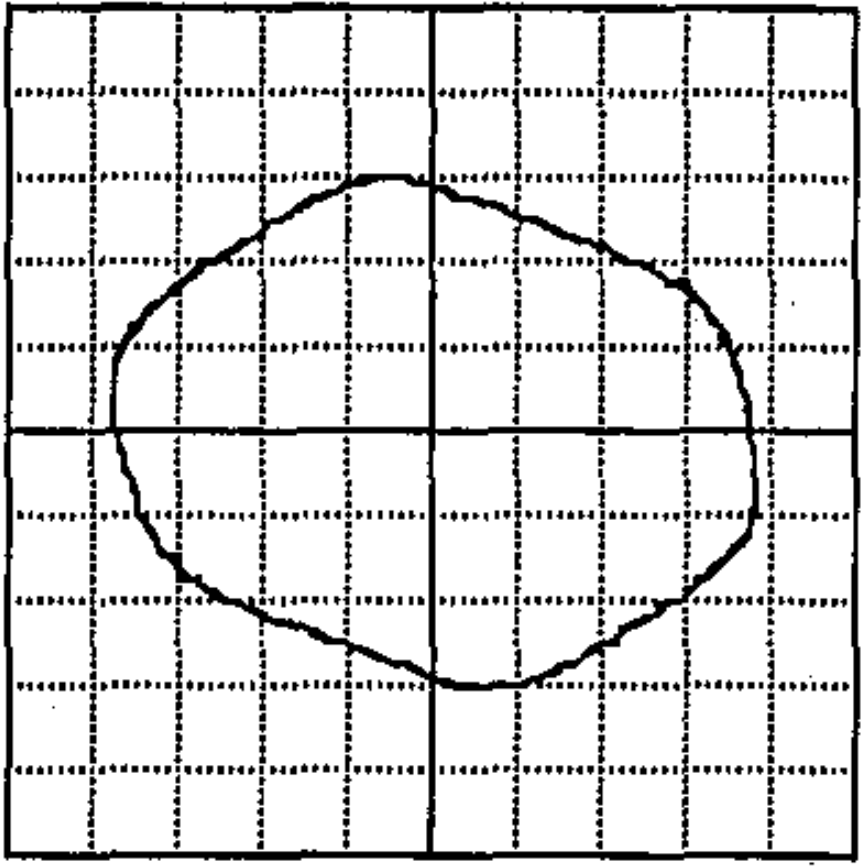
\includegraphics[width=\linewidth]{Parks3.PNG}
    \caption{Shorted Turns}
  \end{subfigure}
  \caption{Park's Vector for experimental current of three-phase, 4 pole, 50 Hz induction motor, reproduced from \cite{MCSA_Parks}\cite{MCSA_Parks2}}
  \label{fig:ParksVector}
\end{figure}

\subsection{Prognostics}\label{sec:prog}

Prognostics is the final element in a complete CBM system.
It provides forecasts about the condition of machines into the future and therefore, crucially, the remaining useful life \cite{CM_randall}.
Having accurate forecasts will increase the effectiveness of maintenance tasks and allow more efficient planning of resources \cite{CBM_overview}.
Improvements in the accuracy of prognostic forecasts have come about as a direct result of increased use of data-driven methods in other fields.
Particularly, Aritificial Intelligence, Machine Learning (ML), Artificial Neural Networks (ANNs), fuzzy logic, unsupervised learing and Expert Systems \cite{CM_dai_gao_2013}.
Many of these techniques have been developed to find correlations in large amounts of data and are now being applied to CBM.
A recently developed machine learning application for denoising images without access to clean references could have an impact in noisy environments where it is hard to measure reference signals, and highlights the potential crossover in machine learning from other applications \cite{Noise2Noise}.
The effective application of data-driven techniques is dependent on the quality of the data and it can be a challenge to obtain training data from commercial applications \cite{CBM_overview}.
A recurring challenge is properly defining system failure, which will vary significantly between applications \cite{CBM_overview}\cite{CM_dai_gao_2013}.
\par

Trend analysis is effective for failures of machines which occur in a gradual and predictable manner \cite{CM_randall}.
The basic concept involves collecting data points over time of a statistic related to the condition of the machine (e.g velocity RMS) and fitting a curve.
By extending the curve, the time to a predetermined failure point can be estimated.
Information about how the curve changes with time can be incorporated into future models as historical data \cite{CBM_overview}.
\par

Another approach is using physics-based models to provide information about how faults will presents themselves.
Examples include crack growth and bearing spalling \cite{CM_randall}.
Both are faults which are hard to verify without causing damage to the machine but can be modelled precisely.
Certain frequencies and patterns can then be looked for as data is collected from the machine.
This approach is being investigated by as part of the projects supported by Lloyd's Register.
\par

Hybrid methods are increasingly leading the way and providing solutions for complex systems which may be operating in unknown environments \cite{CM_dai_gao_2013}\cite{CM_ship_ann}.
Traditional methods such as fault tree analysis and Failure Modes and Effects Analysis (FMEA) have been combined with ANNs to build more accurate and useful CBM systems \cite{CM_ship_ann}.


\section{Condition Monitoring Systems}

Implementing CBM requires having complete CMSs in place.
A complete CMS contains sensors, processors, algorithms, communication channels and human readable outputs.
It is important that such systems are accurate, reliable and work as part of the overall maintenance strategy \cite{CM_mcsa_vib}.
Within the maritime industry, low cost and clear outputs will also be vital to uptake \cite{CBM_beyond_maritime}.


\subsection{Existing Market Solutions}

There are, of course, existing market solutions for CMS.
One industry which has recently become focused on CBM is wind energy generation, due to the poor reliability of early wind turbines \cite{CM_practical_wind_turbine}.
A compilation of commercially available CMS for wind turbines highlights that modern systems are built in much the same way as those designed for relatively simple applications in manufacturing \cite{CM_list_wind_CMS}.
All of the systems surveryed were able to perform at least some level of diagnosis after a fault had occured.
However, there is a large disparity between the capabilities of the systems.
\par
An investigation by Lloyd's Register found that systems can be designed which fulfill the requirements for condition monitoring of marine pumps, but that the cost of such a system can be higher than the cost of the pump itself \cite{LR_cm_systems}.
Single vendor solutions had upfront costs on the order of £10000, with additional costs through installation, licenses and software to follow.
For large segments of the maritime industry, these costs are simply too high.


\subsection{Embedded Systems}

Embedded Systems describes a wide range of systems, generally comprised of microcontrollers with direct access to hardware.
Within the IoT architecture, they are nodes which collect data using sensors, perform processing and transmit data to a central node \cite{Embedded_WSN}.
This approach provides flexibility and speed during deployment at a relatively low cost \cite{Embedded_WSN2}.

\par

There are several key factors which must be considered when designing an embedded CMS for industry:
\begin{itemize}
    \item \textbf{Cost} - While the cost of individual node is low, effective condition monitoring implementations will require many nodes to be placed at different points of the machine or on different machines \cite{Embedded_WSN}\cite{ISO13373-1}. This is a particularly important factor in a cost focused industry such as the maritime industry \cite{CBM_beyond_maritime}. 
    \item \textbf{Processing power} - Powerful systems can use complex analytical tools to perform fault detection and diagnosis quickly, as well as providing more options for communication and interaction \cite{Embedded_ANN}.
    \item \textbf{Security} - There is a growing realisation that security of IoT devices must be enhanced to protect proprietary information and prevent deliberate misuse of devices for malevolent purposes \cite{IoT_security}. 
    \item \textbf{Energy consumption} - Systems which only use small amounts of energy - on the order of 10 mW -  can run independently with energy harvesting methods while sampling sensors in the kilohertz range \cite{Embedded_Energy_Harvesting}.
    \item \textbf{Communication} - There is a wide variety of communication protocols available with different levels of complexity and resilience. Low-energy, wireless protocols such as Bluetooth and Zigbee offer flexibility but could be problematic to implement in noisy environemnts such as ships \cite{Embedded_Comms}.
\end{itemize}

Fig \ref{fig:WSN} shows the software block diagram and built hardware of a wireless embedded system designed to detect faults on motor arrays \cite{VIB_wireless_sensor}.
This represents a typical wireless sensor approach, where data is collected and transmitted to a central unit for further processing.
%In this instance, there are two microcontrollers on the board, one for measuring signals and one for managing the communication.
No processing of the signals is actually performed on board.
\par
The work presented in \cite{Embedded_WSN} and \cite{Embedded_WSN2} demonstrates the potential of embedded systems to process information before transmission.
Both systems are monitoring induction motors, but calculating different parameters.
The system in \cite{Embedded_WSN} monitors all phases of a three phase motor, calculates the RMS current and voltage and transmits information about the power consumed to a central node.
The central node collects data from several wireless sensors and compares it against user-specified limits to determine the condition of the machine.
This work is poorly documented and it is not clear exactly how the embedded software is designed to work or how well the system has been validated.
\par
The system in \cite{Embedded_WSN2} is designed to calculate and transmit the torque, speed and efficiency of the motor.
It shows good agreement between experimental tests and a reference model of the motor.
The embedded software and system architecture is well laid out.


\begin{figure}
  \centering
  \begin{subfigure}[b]{0.49\textwidth}
    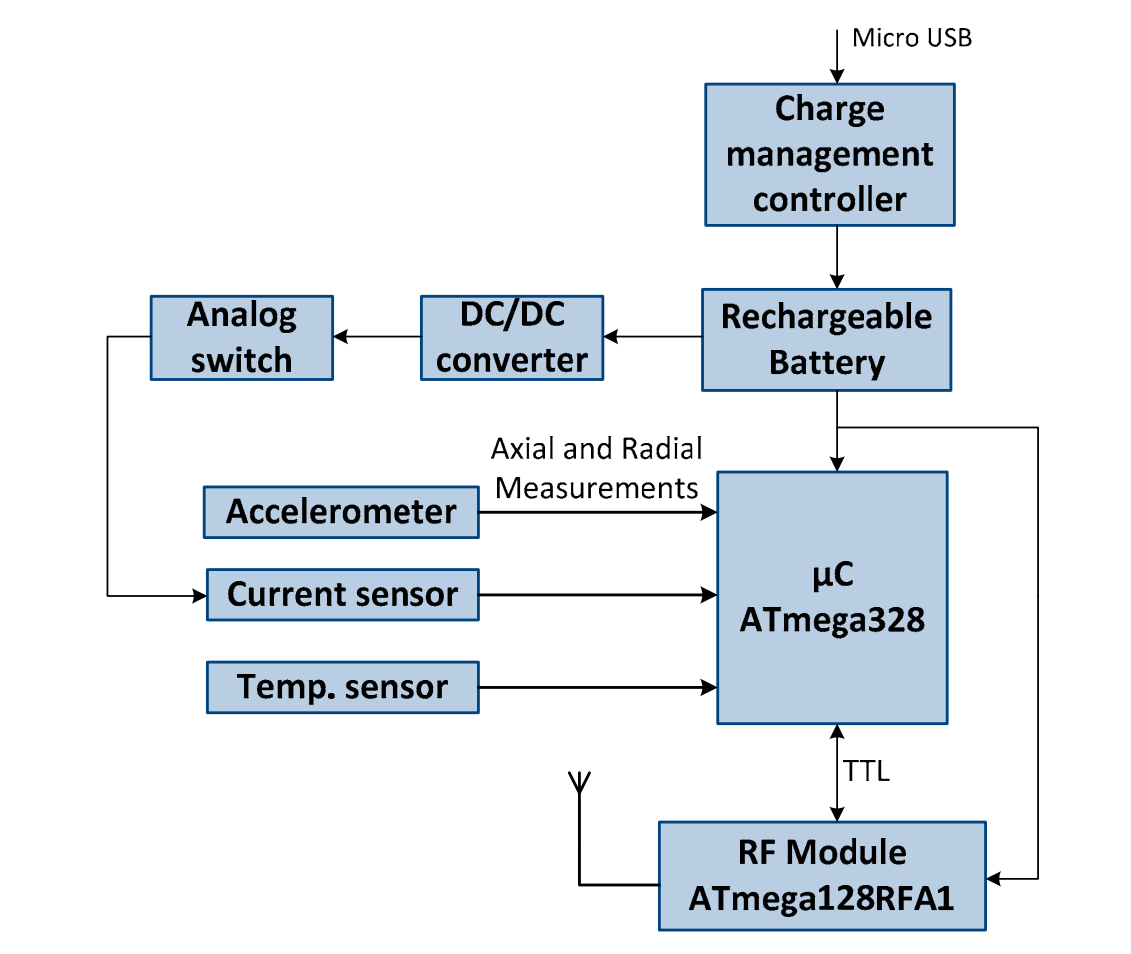
\includegraphics[width=\linewidth]{WSN1.PNG}
    \caption{Block Diagram}
  \end{subfigure}
  \begin{subfigure}[b]{0.49\textwidth}
    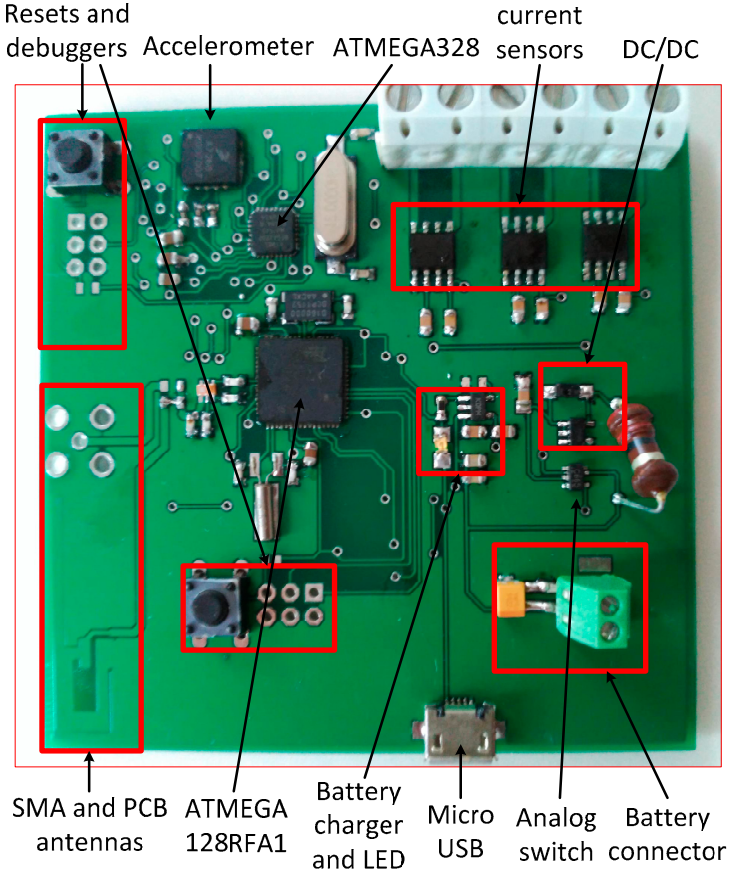
\includegraphics[width=\linewidth]{WSN2.PNG}
    \caption{Photograph of hardware}
  \end{subfigure}
  \caption{Wireless Sensor Node for monitoring and fault detection, reproduced from \cite{VIB_wireless_sensor}}
  \label{fig:WSN}
\end{figure}



